%%
%% The first command in your LaTeX source must be the \documentclass command. This is the generic manuscript mode required for submission and peer review.
\documentclass[manuscript,screen,review]{acmart}

%% Fonts used in the template cannot be substituted; margin 
%% adjustments are not allowed.

%%
%% \BibTeX command to typeset BibTeX logo in the docs
\AtBeginDocument{%
  \providecommand\BibTeX{{%
    \normalfont B\kern-0.5em{\scshape i\kern-0.25em b}\kern-0.8em\TeX}}}

%%
%% For managing citations, it is recommended to use bibliography
%% files in BibTeX format.

%%
%% end of the preamble, start of the body of the document source.
\begin{document}

%%
%% The "title" command has an optional parameter,
%% allowing the author to define a "short title" to be used in page headers.
\title{Improving Presence in Virtual Reality}

%%
%% The "author" command and its associated commands are used to define
%% the authors and their affiliations.
\author{Eliana Laudadio}
\email{elaudadi@rams.colostate.edu}
\affiliation{%
  \institution{Colorado State University}
  \city{Fort Collins}
  \state{Colorado}
  \country{USA}
  \postcode{80521}}

\author{Grant Sinclair}
\email{grantschool.cs@gmail.com}
\affiliation{%
  \institution{Colorado State University}
  \city{Fort Collins}
  \state{Colorado}
  \country{USA}
  \postcode{80521}}
  
\author{Allison Smith}
\email{allison.smith@colostate.edu}
\affiliation{%
  \institution{Colorado State University}
  \city{Fort Collins}
  \state{Colorado}
  \country{USA}
  \postcode{80521}}


%%
%% By default, the full list of authors will be used in the page
%% headers. Often, this list is too long, and will overlap
%% other information printed in the page headers. This command allows
%% the author to define a more concise list
%% of authors' names for this purpose.
\renewcommand{\shortauthors}{Laudadio and Sinclair, et al.}

%%
%% The abstract is a short summary of the work to be presented in the
%% article.
\begin{abstract}
  Presence is one of the key feelings that a virtual reality user depends on to be fully immersed in a virtual environment. This study is interested in understanding the role that audio plays in improving the feeling of presence in virtual reality. A within-subject experiment is ran with three different audio settings to test the level of immersion perceived when a user is in a virtual environment.
\end{abstract}


%%
%% Keywords. The author(s) should pick words that accurately describe
%% the work being presented. Separate the keywords with commas.
\keywords{virtual reality, audio, immersion, presence}


%%
%% This command processes the author and affiliation and title
%% information and builds the first part of the formatted document.
\maketitle

\section{Introduction}
Presence in virtual reality is becoming more and more important as technology exponentially grows beneath our feet. This within-subject study will walk each participant through a virtual world using a VR headset under three different conditions, to test whether different audio stimuli affect the user's feeling of presence in the world. The motivation behind this study is the foundational benefits of virtual reality itself. Virtual reality can be used to “transform education” \cite{SMITH}, relieve surgical patients of pain, and reverse negative stigmas around mental illness. A problem arises as virtual reality becomes more popular, the need to improve its human interaction increases. What is a computer without a mouse; a TV without a remote? Virtual reality without the feeling of being assimilated in a manipulated realm? Presence is a key component to the growth of technology and the user’s experience that comes with it. It is important to seal any cracks in the illusion \cite{CARTER} of this artificial reality in order to avoid ruining the user’s experience, and making the benefits of virtual reality become expendable.  
  

\section{Related Works}

\subsection{Benefits of Virtual Reality}
The motivation for this study comes from an endless range of benefits that virtual reality has to offer. First, what is virtual reality exactly? Virtual reality “is an advanced, human-computer interface that simulates a realistic environment” \cite{Zheng}. In other words, virtual reality holds the capability to seemingly create new worlds and situations for humans to interact with. 

\begin{figure}[ht]
  \centering
  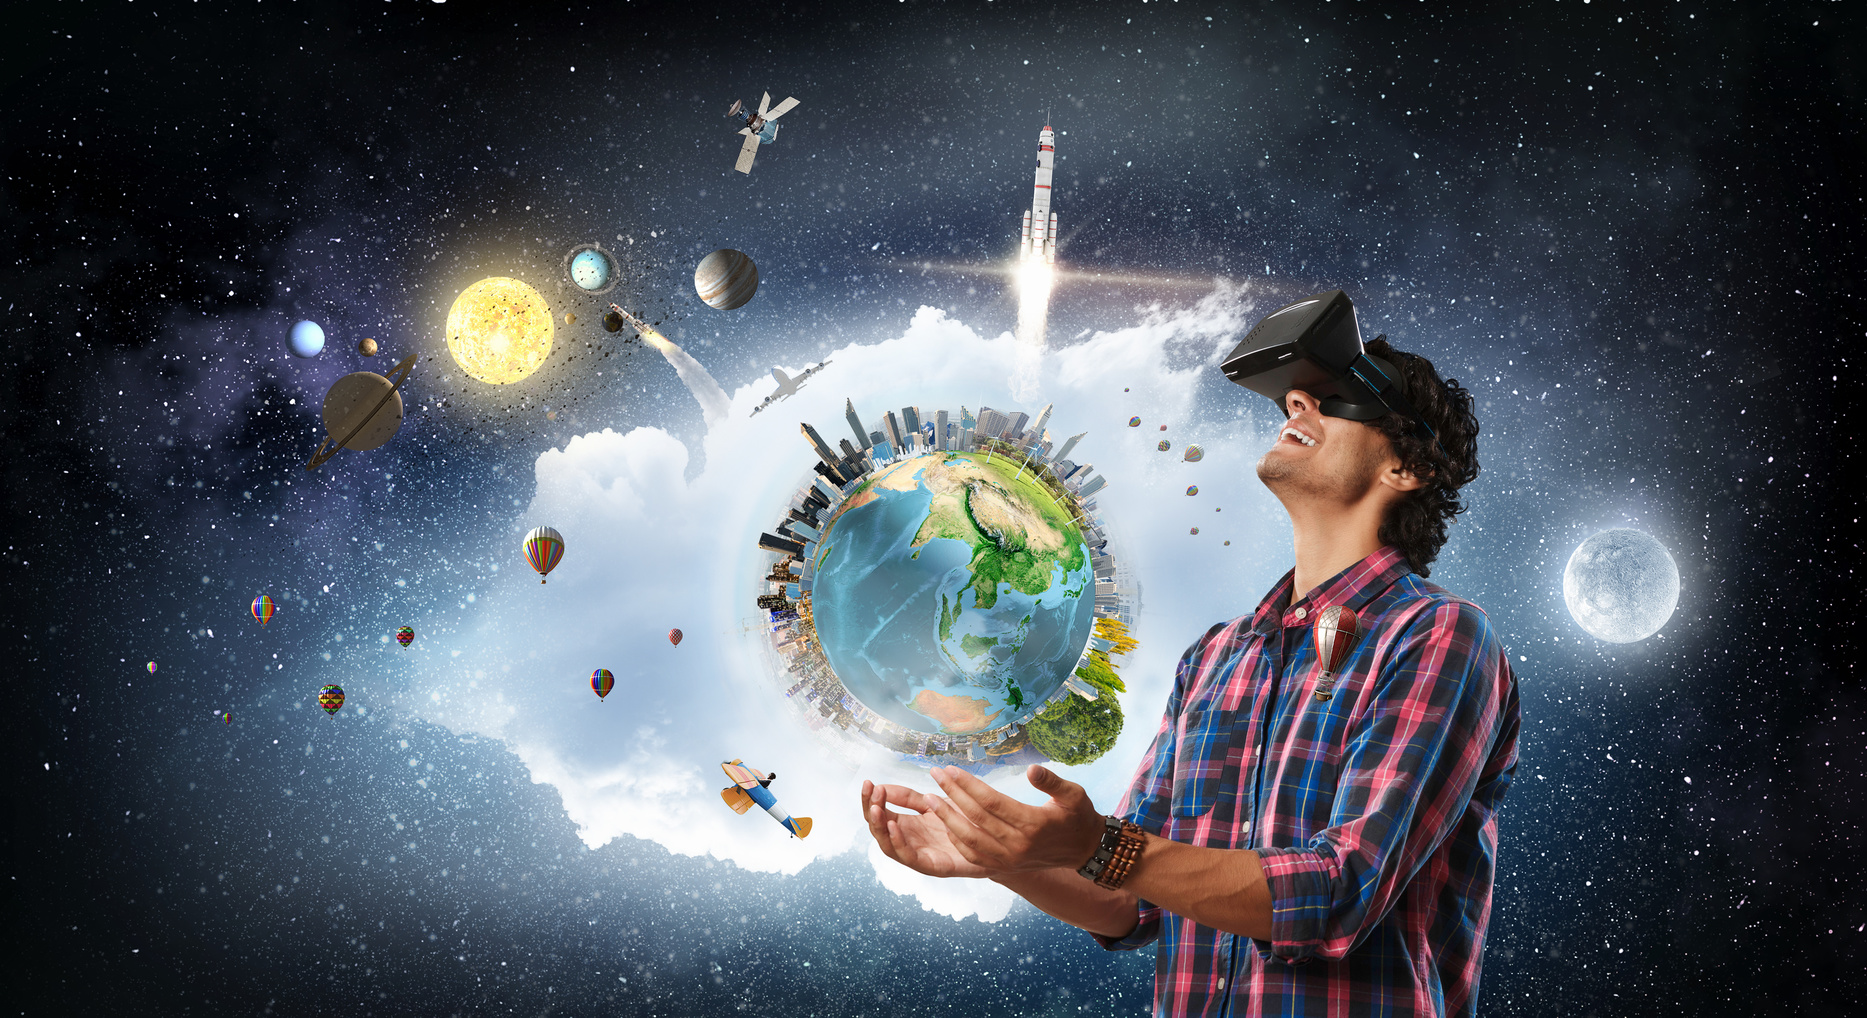
\includegraphics[width=\linewidth]{Virtual_Reality.jpg}
  \caption{Man looking through VR headset at outer-space with the earth, planets, rocket-ship, and satellites. \cite{LYNXPRO}}
  \Description{Man looking through VR headset at outer-space with the earth, planets, rocket-ship, and satellites.}
\end{figure}

The first thing many people may think of when presented with the concept of virtual reality is video games. According to Sage Journals, “virtual reality can provide innovative gaming experiences” that non-immersive gaming consoles such as a desktop computer cannot \cite{PALLAVICINI}. As virtual reality grows and becomes more popular, so will its grasp on a diehard gaming community. However, virtual reality can be used beyond gaming; virtual reality games may provide enough exposure for both mental and physical therapy \cite{SMYS}. Since virtual reality offers physical interaction, physical therapy and rehabilitations have been designed for upper body injuries. As many strokes result in upper limb dysfunction \cite{YATES}], virtual reality may be used as a tool to help a diverse range of patients from injured athletes to stroke patients. 

Furthermore, a study from Science Direct establishes that introducing virtual reality to patients that are in an “excessive pain” during unanesthetized medical procedures may reduce the feeling of pain compared to those who go without the technology \cite{HOFFMAN}. In a study on phobia treatment, the results showed that "virtual reality exposure therapy (VRET)" and in vivo therapy exposure both show positive effects. VRET was better in the presentation of some specific phobias\cite{FREITAS}. This is a common practice in virtual reality to reduce any mental illnesses or phobias with virtual worlds.

This is a new technology that should not be underestimated as educators in all fields can find a use for it in their classrooms. Virtual reality allows history students to witness “historical events first hand” \cite{BOYLES}, it creates a new dimension to having a penpal in a foreign language class as students can seemingly communicate with native speakers face to face. Science students can witness the world of microbiology as if it were proportionate to them. Virtual reality even allows medical students to practice surgeries in a safe environment; the list goes on and it is not limited \cite{BOYLES}. 

Furthermore, in order to reduce the stigma of schizophrenia, final year medical students used to be shown a DVD about a man who had auditory hallucinations \cite{GALLETLY}. While this did work, this topic can be more informative and personal with virtual reality. With the unfortunate fact that many nurses treat schizophrenic patients poorly, another study discusses how the misinterpretation and stigma of schizophrenia results in dramatic hallucinations for schizophrenic patients. Using virtual reality, nurses were exposed to similar hallucinations as their patients, which ultimately resulted in the nurses treating the patients better \cite{FREEMAN}. Creating artificial hallucinations through virtual reality can reduce stigma in schizophrenic patients to where they might even have wholesome hallucinations rather than violent and scary ones. This exhibits that virtual reality is mutually beneficial to not only medical students, doctors, and surgeons, but also to the patients.


\subsection{Why Presence is Important}
From benefits in education to helping mental health patients, virtual reality is an unbelievably strong tool, but what happens if there is a glitch in the illusion or if the user simply doesn't feel present? “For effective Virtual Realities, “presence” is deemed an essential prerequisite” \cite{KERN}; in other words, virtual reality is not virtual reality without presence. A study by Scholar Space exhibited 294 surveys specifying a correlation between immersion and presence while using virtual reality \cite{Mütterlein}. Participants that felt less present in the virtual world they were in, felt less satisfied with virtual reality in general, and this makes sense. 

How satisfied would a user be with a computer if it did not have a mouse? The goal of virtual reality is for the user to forget they are wearing a head mounted display. For this to happen, the user must feel very present in the virtual reality. A human relies heavily on their senses to navigate through their world, and this remains true even in a virtual environment \cite{JELFS}. If a virtual environment only activates one sense, such as a user’s vision (not audio, olfactory, etc), a user’s perceived presence is dramatically decreased \cite{BRINKMAN, JELFS}.

To understand how humans may perceive presence, it is necessary to understand how humans perceive. Cycling through the human factors model \cite{MACKENZIE}, we must unwrap how humans sense a display, in this case, a virtual world. Most humans have five senses being vision, hearing, touch, smell, and taste; the most obvious of these to be used in virtual reality is vision and hearing. 

\begin{figure}[ht]
  \centering
  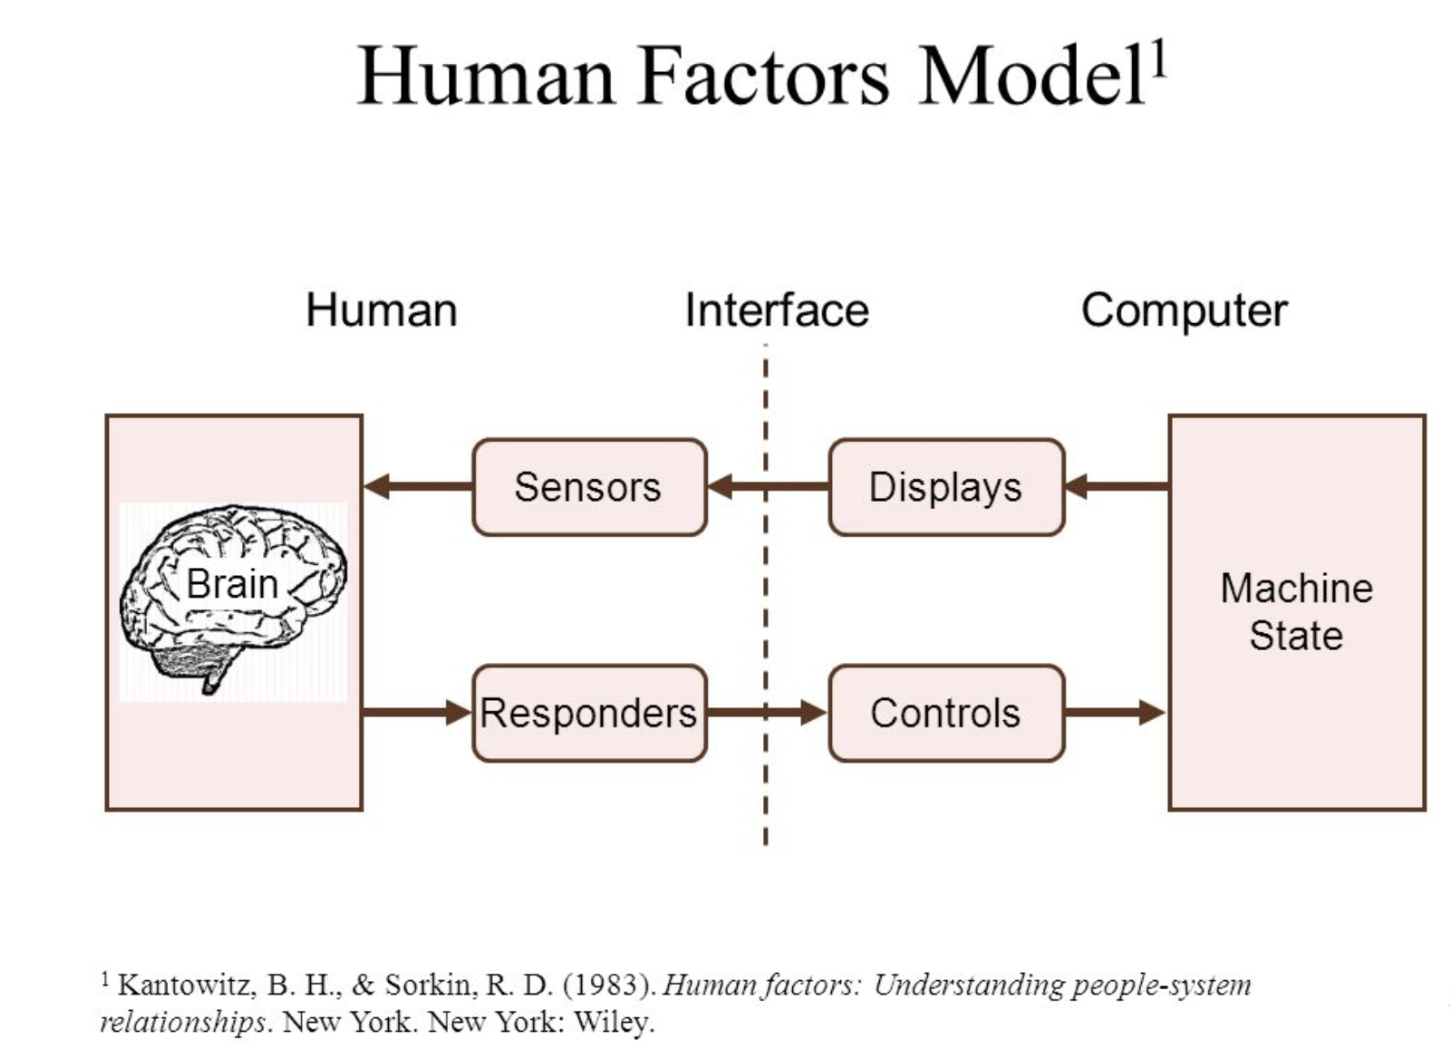
\includegraphics[width=\linewidth]{HumanFactorsModel.png}
  \caption{Human Factors Model \cite{MACKENZIE}}
  \Description{Human Factors Model}
\end{figure}

As far as vision alone in virtual reality, the user is completely encompassed in the new world. At each angle the user may see an entire scene around them that is not physically present, almost as if there were “a television set wrapped itself around their head” \cite{BIOCCA}. A central study in Human-Computer Interaction is the idea of scanpaths, which is the “relationship between eye movements and vision” \cite{HAASS}. This idea is seen previously in websites, where the UI almost psychologically directs the users eyes to specific places on the screen. This is powerful when it comes to immersing the user because it gives the world a natural sense of direction. This brings about questions such as: are the proportions of objects correct? Is the color scheme of the world coherent? Do all of the objects look as if they belong in this world? As people obtain about 80% of their information through the eye \cite{MACKENZIE}, taking visual stimuli in account is a large concern in creating immersion and presence. 

According to ACM Digital Library, “Sound and virtual reality are two important output modalities for creating an immersive '' user experience \cite{ROGERS}. Similarly, while vision is important to feeling presence in a virtual world, a large concern of this paper is how important auditory stimuli are along with a visual world. Source direction, or the “localization” of a sound using two ears \cite{DIETZ}, is a useful way to create auditory immersion. For example, The Virtual Barber Shop is an illusion that makes it to where a user wearing headphones feels like they are physically in a barber shop with only audible stimuli. Sounds coming from the left headphones give a feeling of something actually being to the left of the user \cite{LOVELYVIRUS}. Similarly, sound can be harmonious, meaning it is pleasant, or discordant, meaning that it is unpleasant \cite{MACKENZIE}.  A study by Liverpool University insists that adding discordant sounds to horror movies evokes more of an “emotional tone” from the audience \cite{REDFERN}. Another study measured galvanic skin responses, being physical responses, like sweaty hands , due to emotion, when presented with the soundtrack of scary movies like Jaws. Think about the emotional response directors were trying to create when the famous “Jaws'' sound plays compared to somber music in a sad movie \cite{WILLIAMS}. Sound can make a big difference in immersion on a regular television screen, but how much can it affect a user's experience in a virtual world?

There are definitely some unique studies on how touch, smell, and taste can be incorporated into a virtual world to improve presence, however they are new and strange concepts, and for the most part, will not be discussed in this paper. However, an overall common theme in the experimentation of presence in virtual reality is that “multimodal sensory feedback” increases a “sense of immersion and involvement” for the user \cite{COOPER}. In other words, the more senses that are activated while being immersed in the world, the more the user will feel present. The next part of the human factors model that is of interest to this paper is how the brain perceives such stimuli. Some ways humans perceive the world around them have already been mentioned above; in whether a visual stimulus is familiar or strange and whether an auditory stimulus is harmonious or discordant \cite{MACKENZIE}.

Studies that involve virtual reality and presence are considerably diverse bringing about questions on how virtual worlds affect each user, to how each user may uniquely experience the virtual world. Will the user have a better memory of the world depending on how immersed they were \cite{SMITH}? A study from Stanford “investigated the influence of presence on the memory of virtual environments”. In other words, do virtual environments with more recorded presence improve recall  of the world in participants? \cite{BAILEY} Surprisingly, these last two studies are very similar, but must be broken down. The first study reflects on how presence impacts memory within the virtual world \cite{SMITH}, and the second reflects on whether memory from the virtual world can be taken and used in real life \cite{BAILEY}. This only begins to explore the rabbit hole of studies that can be done to understand just how powerful virtual reality is. In yet another light, presence in virtual reality is subjective, however, can this subjectiveness be perceived similarly by specific personality types? \cite{KOBER} In the previously cited study, participants began with a personality questionnaire before being immersed in a virtual environment. Afterwards, they were asked to complete a presence questionnaire. It was found that there was a correlation between personality type and how immersed the participants felt \cite{KOBER}. As these questions get more and more specific, they intensely recite the importance of presence in virtual reality.

How might our new understanding of perceiving and presence be used to improve the benefits of virtual reality? In an attempt to progress “virtual reality exposure therapy (VRET)”, The National Library of Medicine studied whether the feeling of presence in VR increased the feeling of anxiety. They found that across many different anxiety disorders, the feeling of presence when faced with a triggering object amplified the patient's anxiety \cite{LING}. Being able to correctly mimic or trigger a disorder with VR is important in order to create successful therapies. This is not only for the sake of anxiety disorders, but there are also VR contributions to disorders like autism \cite{STRICKLAND} and PTSD \cite{RIZZO}. Reaching beyond mental illnesses, these therapies can even be created to help reduce anxiety in cancer patients going through chemotherapy \cite{CHOW}. In these virtual worlds it is vital that the user feels present, otherwise there is no reason to pursue these types of therapies as it may discourage patients or increase possible side effects \cite{KNIGHT}.

\begin{figure}[ht]
  \centering
  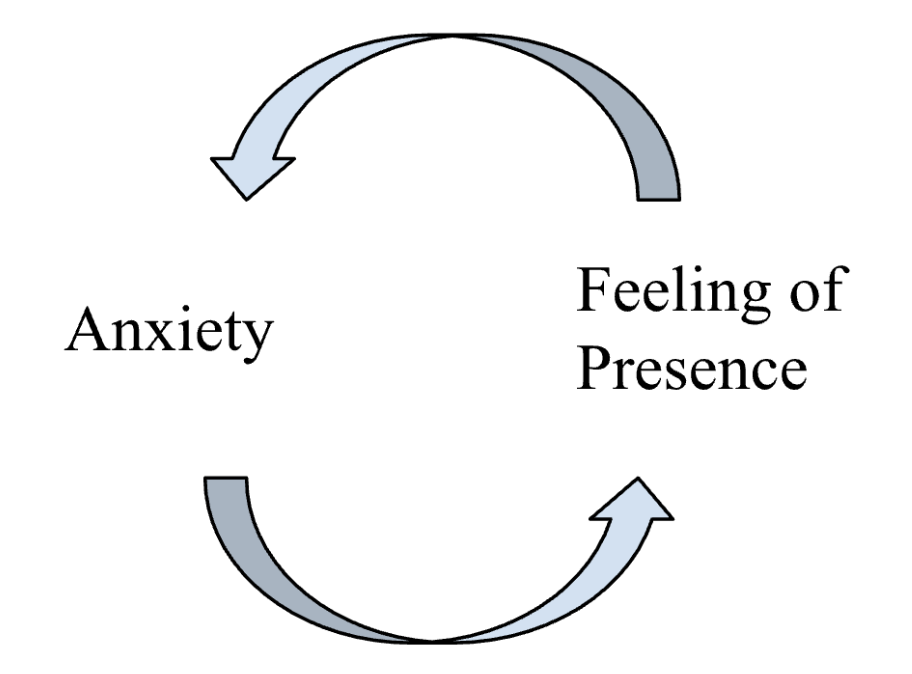
\includegraphics[width=\linewidth]{CycleOfAnxietyAndFeelingOfPresence.png}
  \caption{Cycle of Anxiety and Feeling of Presence}
  \Description{Cycle of Anxiety and Feeling of Presence}
\end{figure}

While presence in virtual reality can cause anxiety as mentioned above, anxiety can also increase the feeling of presence. In a within-between study by MIT Press Direct, participants were put in either an anxiety-inducing or a non-anxiety-inducing environment. Each of the participants had a fear of snakes, so the environment was a virtual ancient Egyptian world. This study tested presence in virtual reality depending on how much anxiety they showed while in an anxiety-inducing virtual world \cite{BOUCHARD}. This exhibits different angles in which the feeling of presence can be increased in a virtual environment. 

Immersion is dependent on the user being able to navigate and understand the virtual environment. A user will evaluate the plausibility of the environment and  ask questions like: Does the environment respond to my movements? Is the story coherent in itself? Does the sequence of events make sense? \cite{WEBER}. 

The answers to these questions determine the level of perceived reality. Virtual reality needs a sense of immersion and presence in order for the user to feel satisfied with the system. Without presence in virtual reality, its many benefits lose value; so a priority in virtual reality is to understand how presence can be increased. Activating a user’s senses (in addition to vision) is a great way to increase the user’s sense of presence. 


 
\subsection{Similar Studies}
As mentioned above, research specifying presence in virtual reality can branch off in countless directions, however in this paper we are simply studying the effect of audio on a user's perceived presence in virtual reality. Below are some similar studies that will give an idea of what our research is trying to capture. Along with that, a small review will be provided on how researchers are gathering results based off of cognitive studies similar to this.

Firstly, a within-subjects study by SpringerLink put participants in a virtual kitchen and asked them how present they felt in the virtual environment depending on whether or not there was a physical odor exposed to the subject. This study found that the subjects felt more present in the virtual kitchen when they were exposed to an odor \cite{BAUS}. This study is a good example of perceiving the sense of smell. Something interesting about this study is that the researchers put the subjects in a physical environment and surrounded them with physical odor as they also exposed the subjects to a virtual environment. Overall, this is an interesting topic as many studies examine that adding smell to virtual systems increases presence. Unfortunately, however, technology currently does not have the “hardware to produce olfactory stimulation” \cite{ZYBURA}, it is interesting to see how researchers are finding ways to study its significance.

In another study called “The sound of Being There”, studied how different auditory illusions created more presence in the exposed world. Similar to the Virtual Barber Shop, this study created “illusions of place”, making the subject feel like they were visually in a new location, “illusions of plausibility”, making the subject feel like they were mentally in a new location, and finally, “virtual body ownership”, making the subject feel like their virtual body is their real body. With these three frameworks, the researchers examined presence in a virtual world by combining visual and auditory stimuli \cite{NORDAHL}.

Audio feedback is one of the most important features in virtual reality that engender a sense of presence \cite{JELFS}. However, not all audio has the same impact. It was found that a low-quality, single-source audio is less immersive than a high-quality, layered audio \cite{BRINKMAN}. On a similar note, not all virtual reality videos have the same impact on presence. As can be expected, a higher-quality video increases feelings of immersion, realism, and enjoyment over a low-quality video \cite{LEVEE}. With this understanding that activating a user’s senses increases their feelings of presence in a virtual reality environment, we are seeking to explore the impact of overlaying multiple audios on a user’s perceived presence. 

Considering each study that has been evaluated here thus far, how might one measure a cognitive gradient such as feeling present? Tina Wu describes presence as a unit to measure response levels. In this study, participants were asked to ride a roller coaster in a virtual environment. The response levels in this study include swaying with the roller coaster, motion sickness, and posture \cite{Wu}. The state of the study depended on the responses to the roller coaster in different realms of immersion. Other experiments will use surveys at the end of their studies directly asking the participants how they felt in the world, among other relevant debriefings \cite{SCHUEMIE}. Some studies are simple questionnaires asking participants what makes them feel more present on a likert scale in preparation to create a virtual world \cite{WITMER}. 

Overall, an empowering conclusion within these related works is that there is a “lack of standardization” \cite{BOSMAN} in auditory virtual reality. In an area of study that may produce endless benefits, it is important to solidify standardizations. The underlying goal in this paper is to be one step closer to creating an understanding of presence in virtual reality by incorporating audio into virtual worlds, and maybe hint at a future of virtual worlds with multiple sensory inputs.



\section{Methodology}
In human-computer interaction, people's presence in virtual reality is very important. In order to collect people's reactions to virtual reality, we randomly found subjects and let them experience their presence in VR during three phases, collected their reactions at each phase, provided surveys for subjects to complete after each phase, and analyzed the data generated at each phase. 


\subsection{Experiment Design}
Our prototype is a Virtual Reality landscape with a waterfall, rocks, trees, and a walking path that can be viewed by our subjects via a virtual reality headset, as shown in Figure 1. The program is written in C\#, HLSL, and ShaderLab. Our independent variable is the use of audio in virtual environments with three auditory conditions played over a waterfall scene. Our dependent variable is the level of immersion and presence each subject feels at each condition.


\begin{figure}[ht]
  \centering
  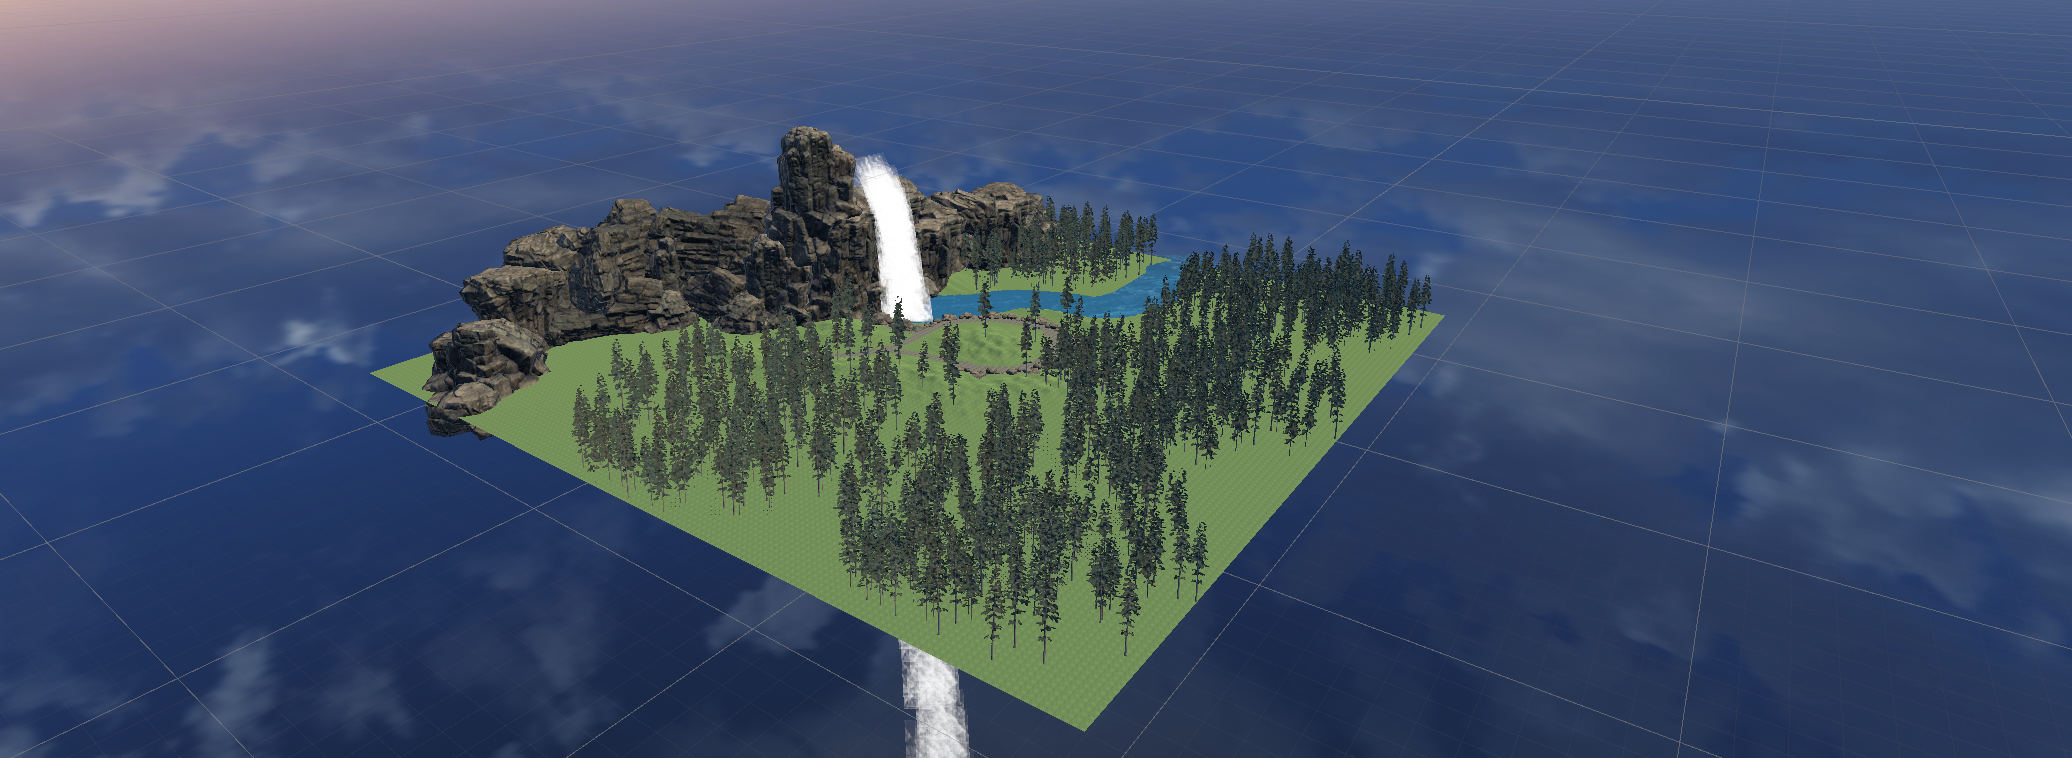
\includegraphics[width=\linewidth]{CP2-world.png}
  \caption{Snapshot of a virtual environment with waterfall, rocks, trees, grass, and a walking path.}
  \Description{Snapshot of a virtual environment with waterfall, rocks, trees, grass, and a walking path.}
\end{figure}
	

This study uses within-subjects design so each subject is tested on all conditions, which are as follows:

\begin{enumerate}
    \item No sound in the virtual environment
    \item Only mixed forest/ambient audio played while subject is in the virtual environment
    \item Waterfall audio with mixed forest/ambient audio played while subject is in the virtual environment
\end{enumerate}

Each trial started with the subject filling out an introduction survey to gather their experience with VR and some other points of information. We then used our research script to instruct the subject on exactly what to do during their trial. We used a 3x3 Latin Square to change the order of administering test conditions between subjects to reduce the chance of a learned effect. Next, the subject put on the VR headset and ran through the first test condition. We chose to note the subjects' vocal reactions (if any) to viewing the waterfall. After the condition was tested, we had the subject remove the headset and gave them a survey asking about their feeling of presence while in the virtual environment. We didn’t have the subject fill out the questionnaires while within the virtual environment because it doesn’t achieve more accurate results \cite{THAKKAR}. Repeating the same steps, we had the subject put the headset back on, run condition two, then fill out another survey, and repeat for condition three. After all conditions were complete, we had the subjects fill out an exit survey. 

\subsection{Experiment Execution}
We conducted the study on 16 different collegiate peers with different backgrounds. After having the participant fill out the consent form, they were asked to put on the VR headset and start their first trial. After their trial we asked them to fill out our survey which asked the following questions based on a Likert scale from 1-5: 

\begin{enumerate}
  \item How present did you feel in the virtual environment? (Presence)
  
  \item How much did the visual aspects of the environment immerse you? (Visual Immersion)
  
  \item How much did the audio aspects of the environment immerse you? (Audio Immersion)
  
  \item How much did your experiences in the virtual environment seem consistent with your real-world experiences? (Real-world Consistency)

  \item How much did the audio aspects distract you during your virtual reality experience? (Audio Distraction)

  \item How involved were you in the virtual environment experience? (Involvement)

  \item How quickly did you adjust to the virtual environment experience? (Adjustment Speed)

  \item How well could you concentrate on the assigned tasks or required activities rather than on the mechanisms? (Task Concentration)
  
\end{enumerate}

After the subject finished the survey we had them put the VR headset back on, run trial 2, then fill out the survey again, and repeat the same steps for trial 3. 


\section{Results}
After executing all of the experiments we were able to aggregate the data by trial and find the average values for each question. Figure 5, 6, and 7 shows the data results from Trial 1, 2, and 3, respectively, with the average scores per question at the bottom.

\begin{figure}[ht]
  \centering
  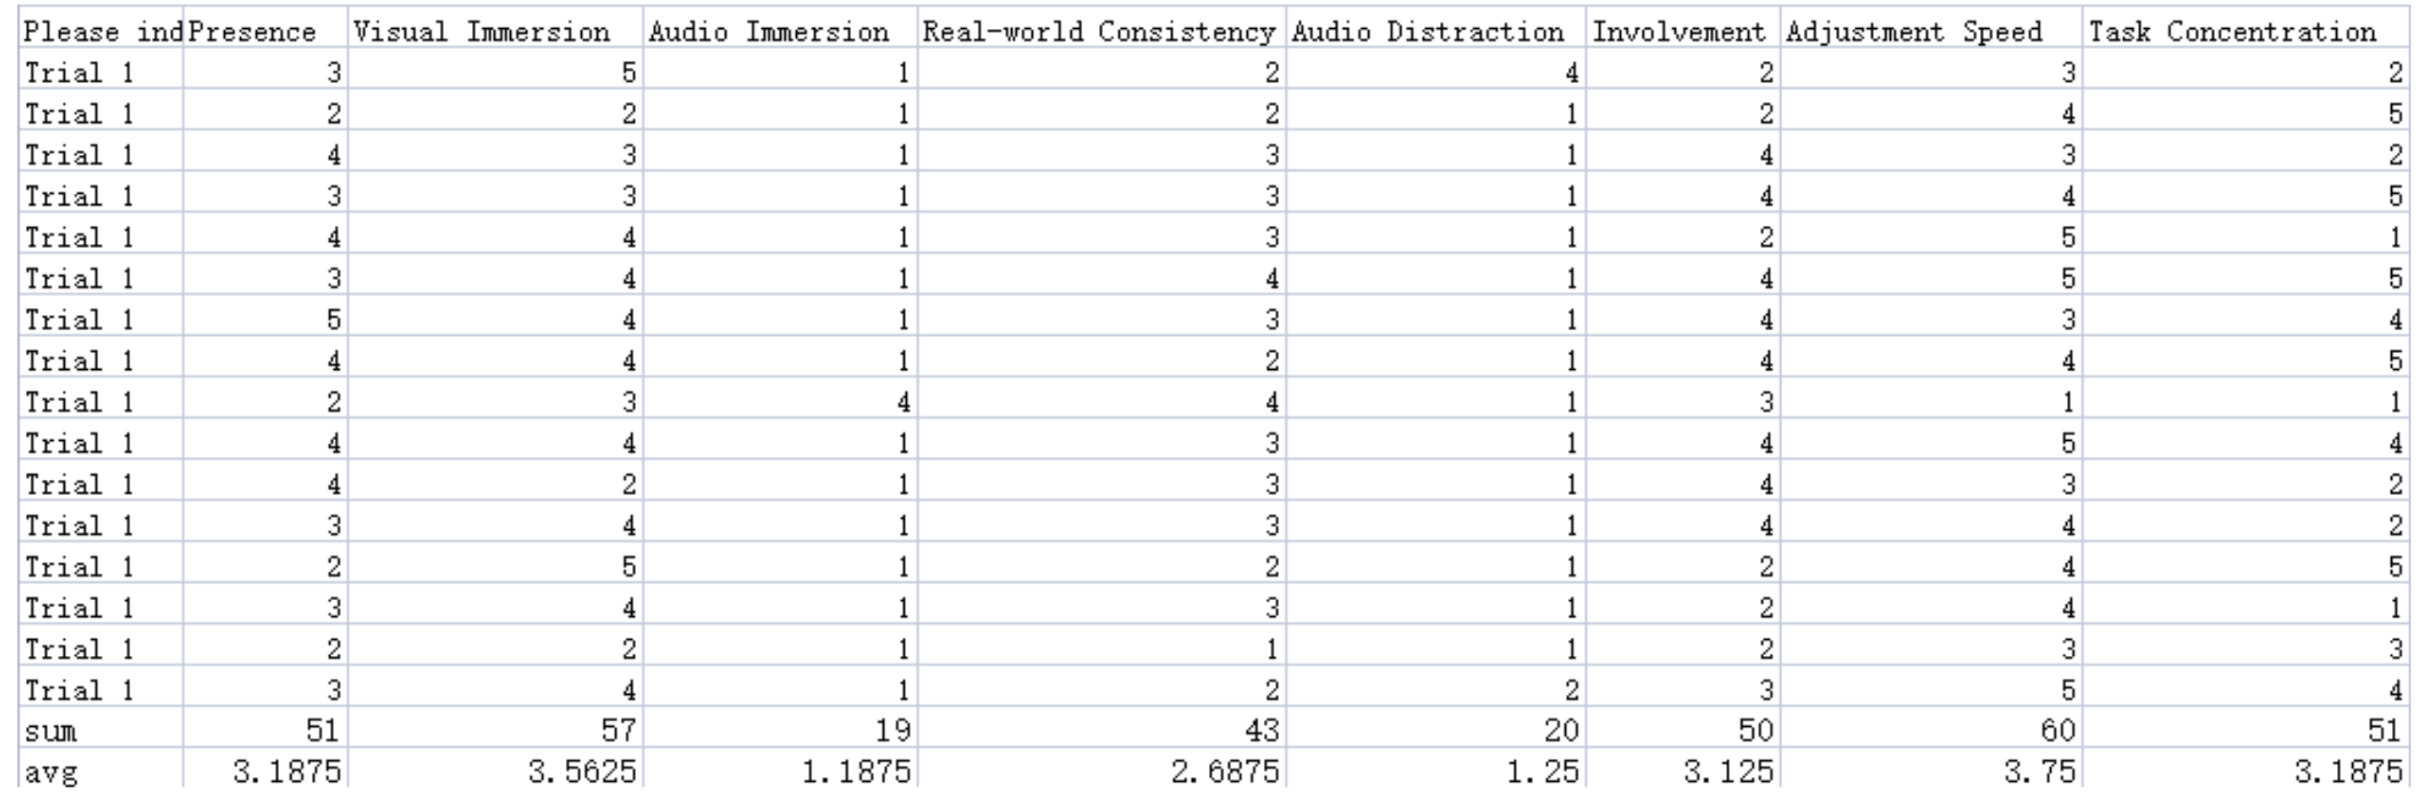
\includegraphics[width=\linewidth]{trial1.png}
  \caption{Trial 1: No sound in the virtual environment}
  \Description{Excel spreadsheet of Trial 1: No sound in the virtual environment}
\end{figure}


\begin{figure}[ht]
  \centering
  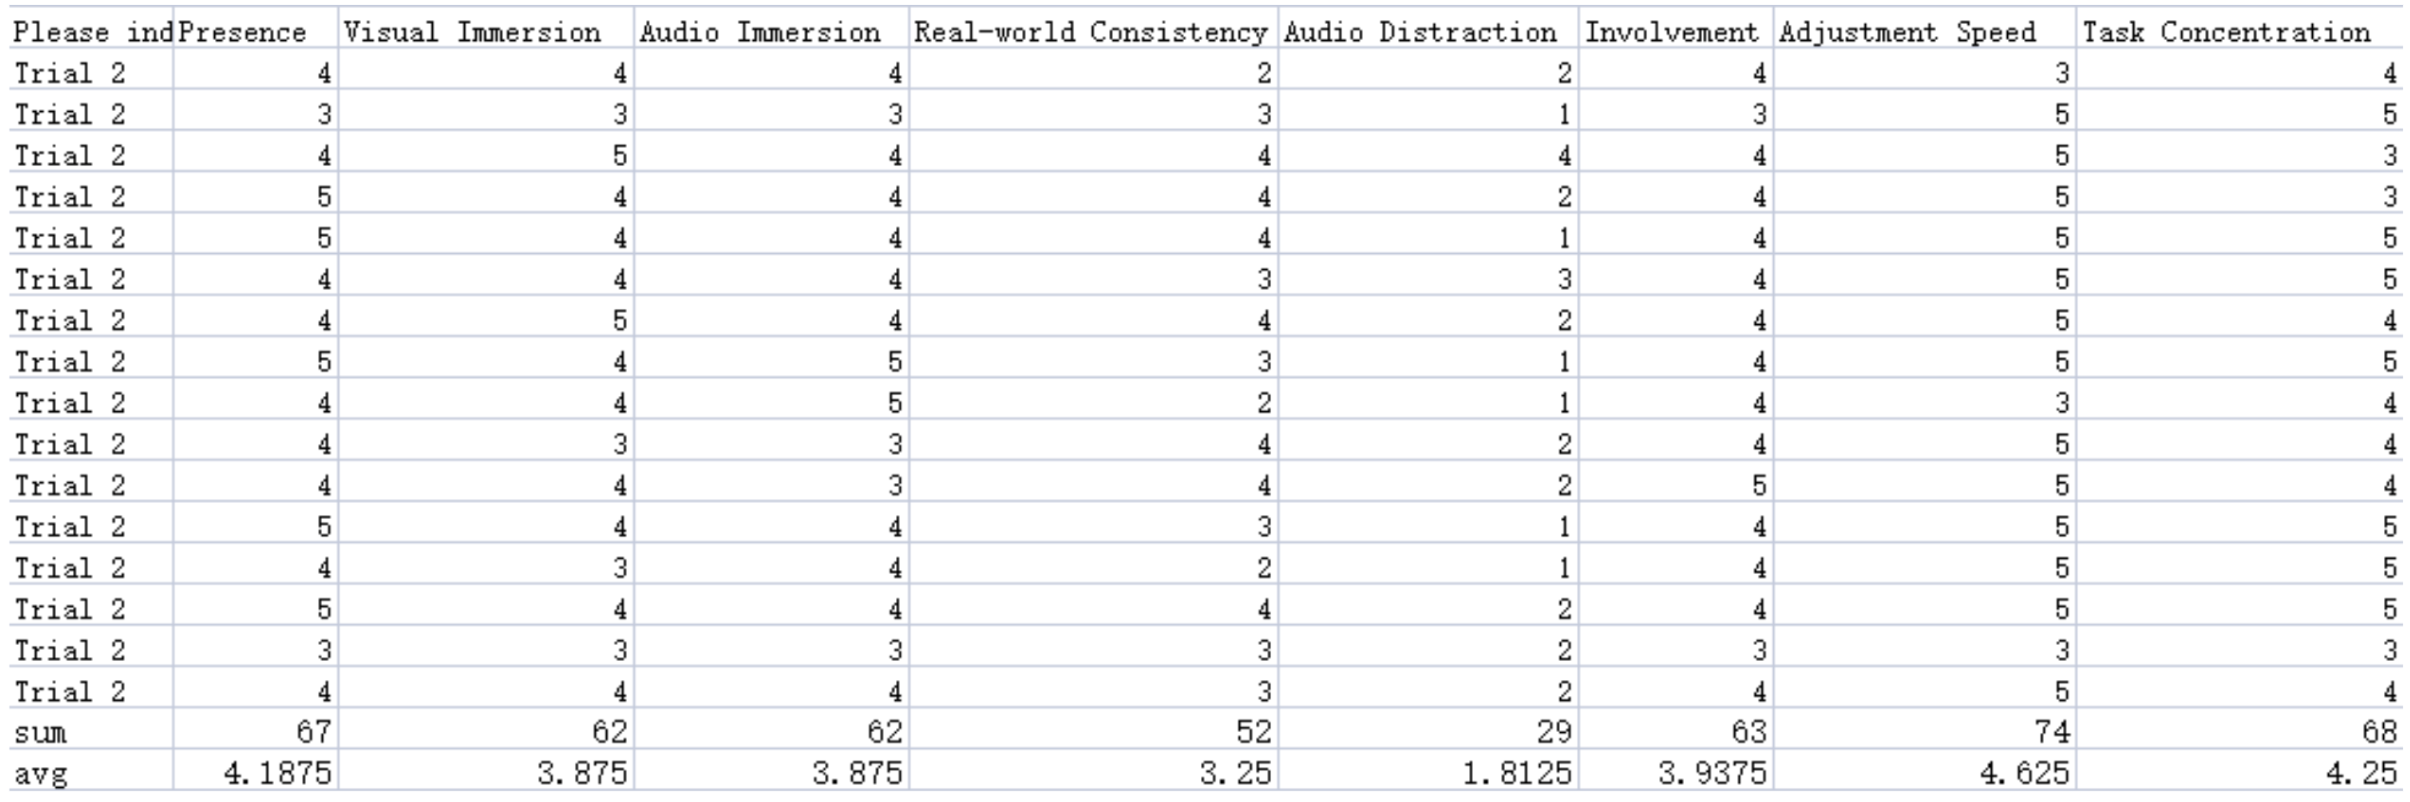
\includegraphics[width=\linewidth]{trial2.png}
  \caption{Trial 2: Only mixed forest/ambient audio played while subject is in the virtual environment}
  \Description{Excel spreadsheet of Trial 2: Only mixed forest/ambient audio played while subject is in the virtual environment}
\end{figure}


\begin{figure}[ht]
  \centering
  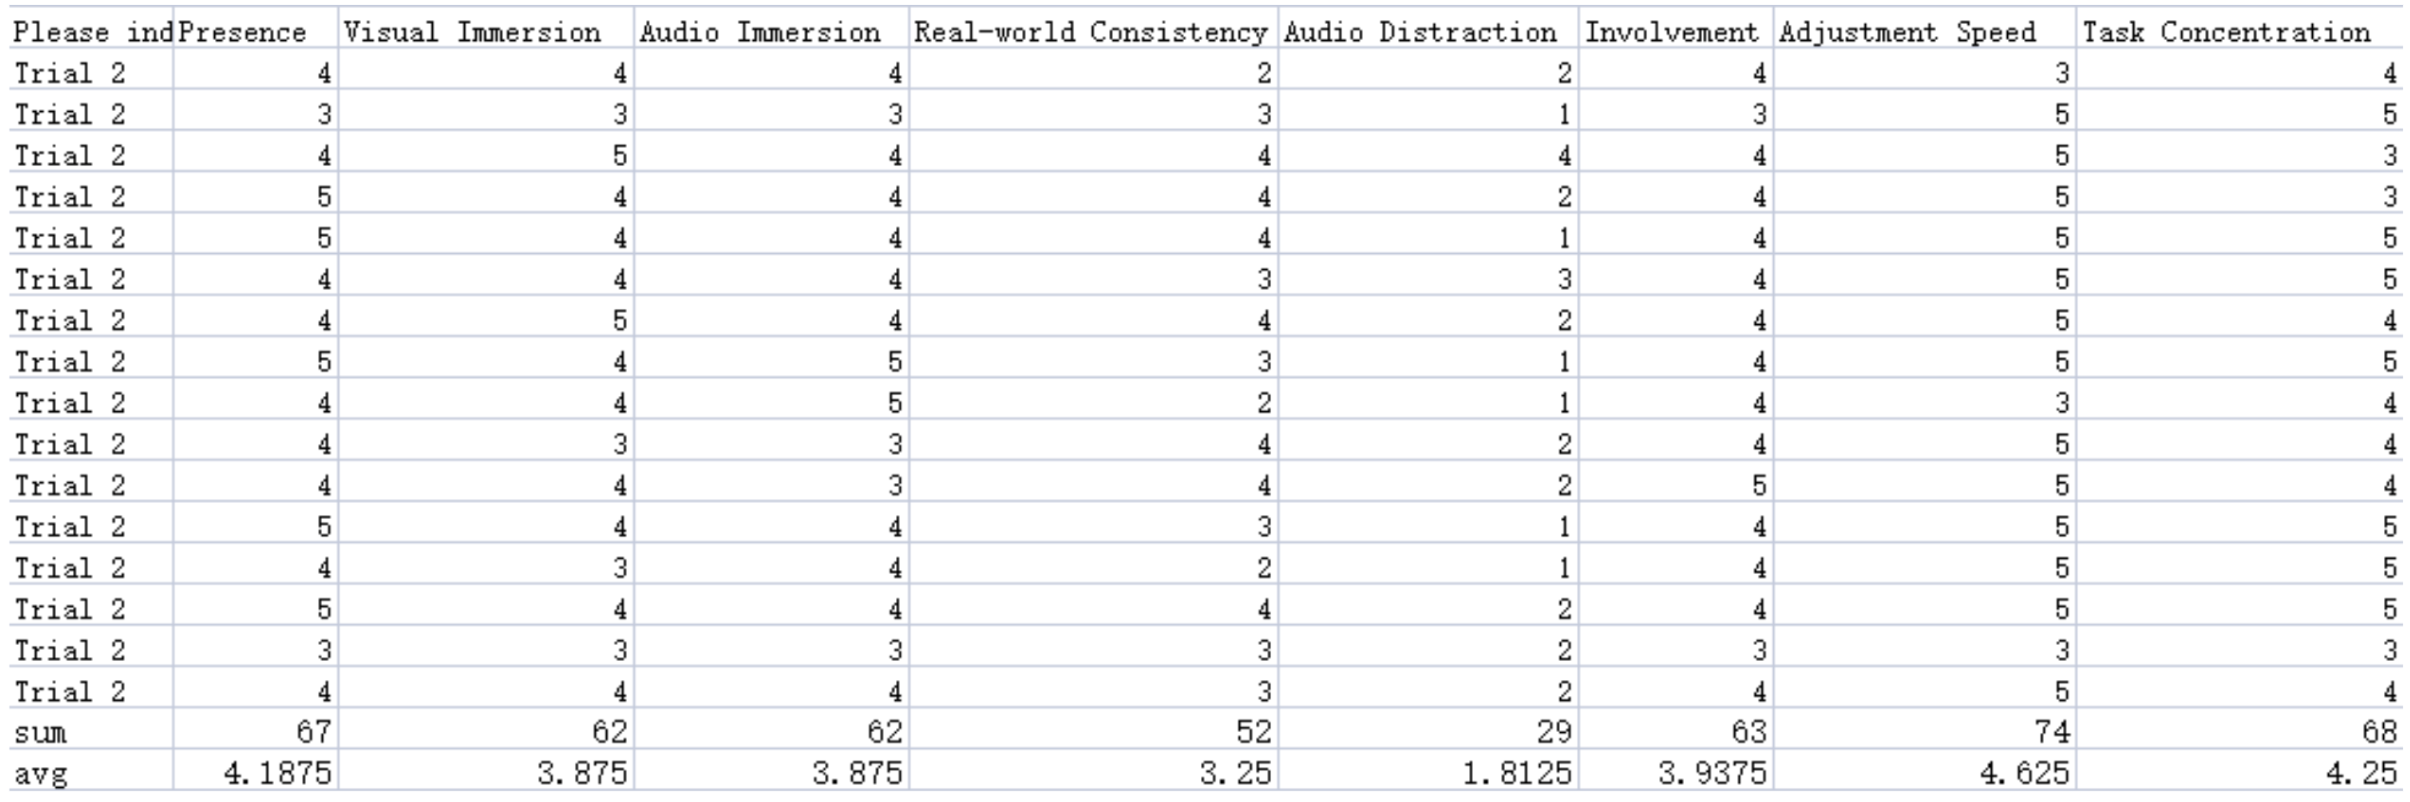
\includegraphics[width=\linewidth]{trial2.png}
  \caption{Trial 3: Waterfall audio with mixed forest/ambient audio played while subject is in the virtual environment}
  \Description{Excel spreadsheet of Trial 3: Waterfall audio with mixed forest/ambient audio played while subject is in the virtual environment}
\end{figure}





The average scores for presence, visual immersion, audio immersion, real-world consistency, involvement, adjustment, and concentration increased from Trial 1 to Trial 3. This suggests that the addition of water and nature sounds in the virtual environment enhanced the users' sense of presence and immersion, making their experiences feel more realistic and engaging.
Comparing Trial 2 and Trial 3, the inclusion of nature sounds alongside water audio further improved the sense of presence, audio immersion, and real-world consistency. This indicates that a more diverse and layered audio environment can significantly contribute to a more immersive and authentic virtual reality experience.
Moreover, it is important to note that the average scores for audio distraction were lowest in Trial 1 and highest in Trial 3. This indicates that while more complex audio environments can enhance the overall experience, they may also introduce potential distractions. However, the overall increase in presence, immersion, and involvement suggests that the benefits of adding audio elements outweigh the potential distractions in creating a more engaging and realistic virtual reality experience.

To better analyse the data we ran an ANOVA on each question across the three trials. 

Figure 8 shows the ANOVA table for Question 1. The effect of audio on presence was statistically significant (F(2, 30) = 28.049, p < .0001).


\begin{figure}[ht]
  \centering
  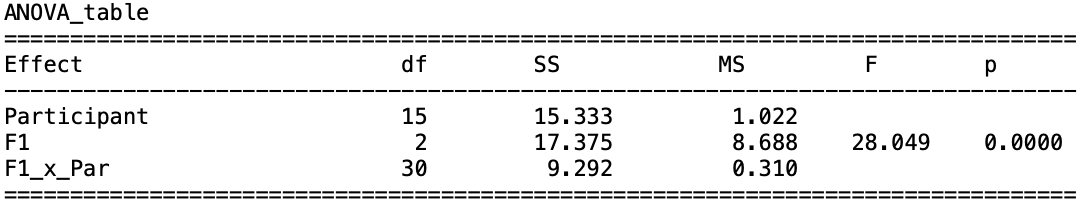
\includegraphics[width=\linewidth]{Q1ANOVA.png}
  \caption{ANOVA for Question 1:  How present did you feel in the virtual environment? (Presence)}
  \Description{ANOVA for Question 1: How present did you feel in the virtual environment? (Presence)}
\end{figure}


Figure 9 shows the ANOVA table for Question 2. The effect of audio on visual immersion was not statistically significant (F(2, 30) = 1.260, p > .05).

\begin{figure}[ht]
  \centering
  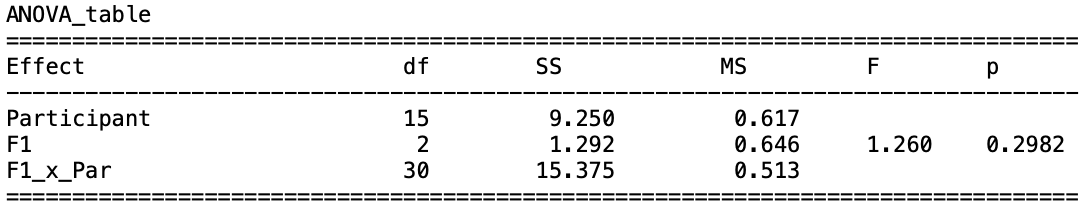
\includegraphics[width=\linewidth]{Q2ANOVA.png}
  \caption{ANOVA for Question 2:  How much did the visual aspects of the environment immerse you? (Visual Immersion)}
  \Description{ANOVA for Question 2: How much did the visual aspects of the environment immerse you? (Visual Immersion)}
\end{figure}



Figure 10 shows the ANOVA table for Question 3. The effect of audio on audio immersion was statistically significant (F(2, 30) = 220.886, p < .0001).

\begin{figure}[ht]
  \centering
  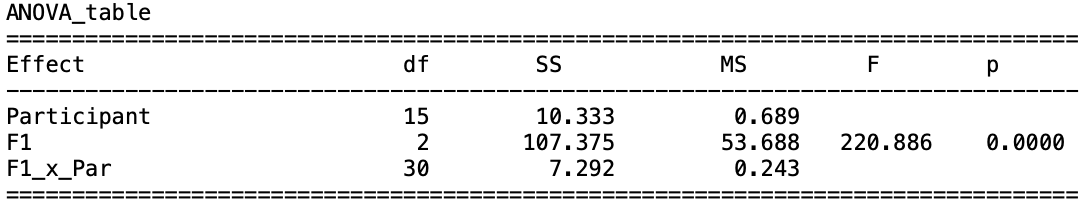
\includegraphics[width=\linewidth]{Q3ANOVA.png}
  \caption{ANOVA for Question 3:  How much did the audio aspects of the environment immerse you? (Audio Immersion)}
  \Description{ANOVA for Question 3: How much did the audio aspects of the environment immerse you? (Audio Immersion)}
\end{figure}



Figure 11 shows the ANOVA table for Question 4. The effect of audio on real-world consistency was statistically significant (F(2, 30) = 12.664, p < .0005).

\begin{figure}[ht]
  \centering
  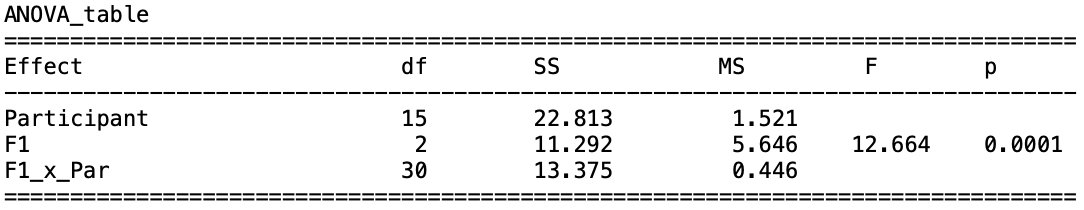
\includegraphics[width=\linewidth]{Q4ANOVA.png}
  \caption{ANOVA for Question 4:  How much did your experiences in the virtual environment seem consistent with your real-world experiences? (Real-world Consistency)}
  \Description{ANOVA for Question 4: How much did your experiences in the virtual environment seem consistent with your real-world experiences? (Real-world Consistency)}
\end{figure}


Figure 12 shows the ANOVA table for Question 5. The effect of audio on audio distraction was not statistically significant (F(2, 30) = 3.223, p > .05).

\begin{figure}[ht]
  \centering
  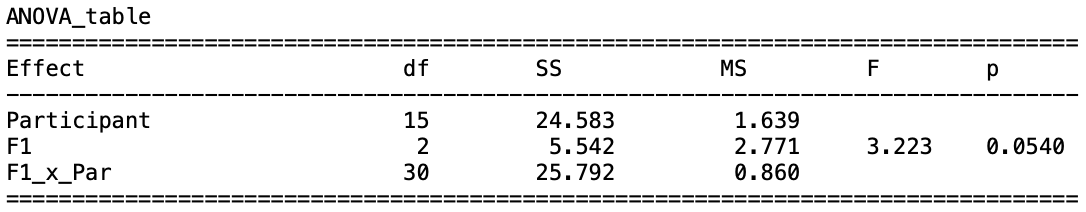
\includegraphics[width=\linewidth]{Q5ANOVA.png}
  \caption{ANOVA for Question 5:  How much did the audio aspects distract you during your virtual reality experience? (Audio Distraction)}
  \Description{ANOVA for Question 5:  How much did the audio aspects distract you during your virtual reality experience? (Audio Distraction)}
\end{figure}


Figure 13 shows the ANOVA table for Question 6. The effect of audio on involvement was statistically significant (F(2, 30) = 18.466, p < .0001).

\begin{figure}[ht]
  \centering
  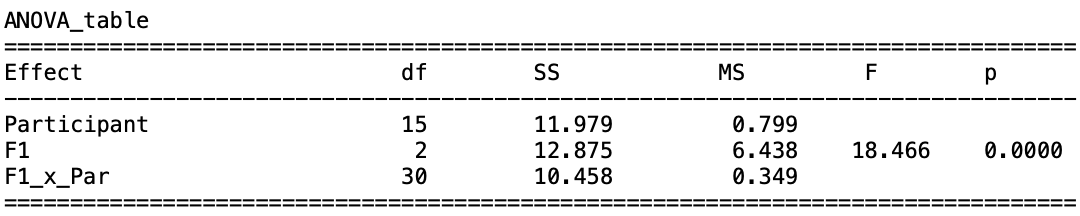
\includegraphics[width=\linewidth]{Q6ANOVA.png}
  \caption{ANOVA for Question 6:  How involved were you in the virtual environment experience? (Involvement)}
  \Description{ANOVA for Question 6:  How involved were you in the virtual environment experience? (Involvement)}
\end{figure}


Figure 14 shows the ANOVA table for Question 7. The effect of audio on adjustment speed was statistically significant (F(2, 30) = 18.191, p < .0001).

\begin{figure}[ht]
  \centering
  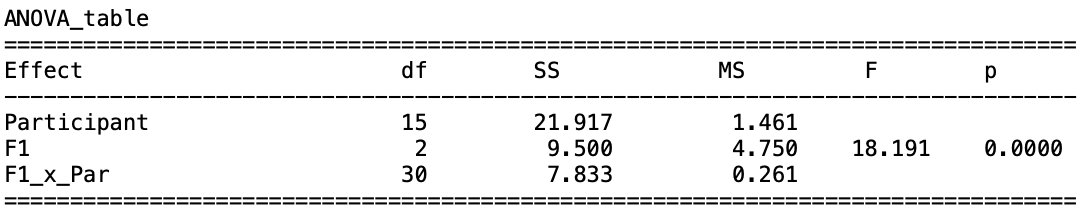
\includegraphics[width=\linewidth]{Q7ANOVA.png}
  \caption{ANOVA for Question 7:  How quickly did you adjust to the virtual environment experience? (Adjustment Speed)}
  \Description{ANOVA for Question 7:  How quickly did you adjust to the virtual environment experience? (Adjustment Speed)}
\end{figure}



Figure 15 shows the ANOVA for Question 8. The effect of audio on task concentration was statistically significant (F(2, 30) = 9.242, p < .001).

\begin{figure}[ht]
  \centering
  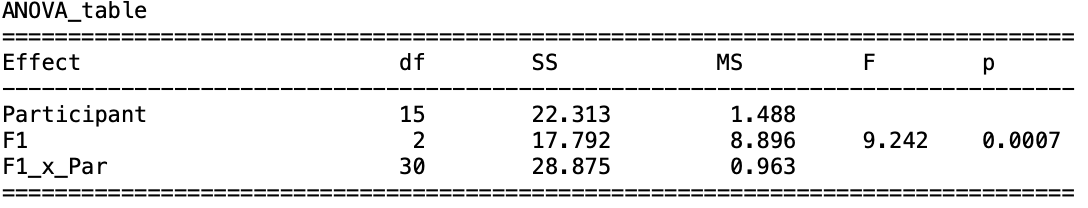
\includegraphics[width=\linewidth]{Q8ANOVA.png}
  \caption{ANOVA for Question 8:  How well could you concentrate on the assigned tasks or required activities rather than on the mechanisms? (Task Concentration)}
  \Description{ANOVA for Question 8:  How well could you concentrate on the assigned tasks or required activities rather than on the mechanisms? (Task Concentration)}
\end{figure}



\section{Conclusion and Future Work}
The goal of this project is to understand the importance of audio in virtual reality in order to increase the feeling of presence in users. Without presence in virtual reality, the benefits it offers in fields such as medical and education become useless. Specifically, studies on audio and presence in virtual reality are limited leaving a lack of standardization within that branch.  In this study we created a virtual environment that included a walk through a forest and past a waterfall. Each participant walked through the virtual environment three times with either no audio, the sound of the waterfall, or the sound of the waterfall with natural noises. After running an ANOVA of our results we found that the inclusion of audio does have a statistically significant effect increasing the user’s feeling of presence in the virtual environment. This study offers a baseline standardization of audio in this new technology that has the potential to improve any and every field.



%%
%% The acknowledgments section is defined using the "acks" environment
%% (and NOT an unnumbered section). This ensures the proper
%% identification of the section in the article metadata, and the
%% consistent spelling of the heading.
\begin{acks}
To our participants, for helping us gather great research on improving presence in virtual reality.
\end{acks}

%%
%% The next two lines define the bibliography style to be used, and
%% the bibliography file.
\bibliographystyle{ACM-Reference-Format}
\bibliography{team-bibliography}

%%
%% If your work has an appendix, this is the place to put it.
\appendix



\end{document}
\endinput
%%
%% End of file 
